% Οι άνθρωποι γνωρίζουν τα γινόμενα.
% Τα μέλλοντα γνωρίζουν οι θεοί,
\dictum[The Iliad of Homer, Book I]{
  Tis time to save the few remains of war. \\
  But let some prophet, or some sacred sage, \\
  Explore the cause of great Apollo's rage; \\
  Or learn the wasteful vengeance to remove}

\begin{summary}
\item FluiDB is well suited for join-heavy star schemata so we
  evaluated using the SSB-TPC-H benchmark.
\item Our evaluation shows that FluiDB is able to plan around the
  space constraints and come up with plans that materialize
  intermediate results that are useful for future queries.
\item FluiDB is generally faster than the baseline due to caching but
  at times may be slower in individual queries when it receives
  ``unexpected'' queries.
\item FluiDB generally performs better when allowed larger memory
  budgets but this speedup is based on heuristic assumptions that
  sometimes break in interesting ways.
\end{summary}

We based our evaluation of FluiDB on the Star Schema Benchmark (SSB)
\cite{barataOverviewDecisionSupport2015} which is a variation of
TPC-H. Like TPC-H it models the data warehouse of a wholesale
supplier.

As the name suggests, these queries query a star schema. The star
schema is derived from the TPC-H schema (figure \ref{fig:tpch_schema})
by merging the \sql{linenumber}, \sql{orders} and
\sql{partsupp} and completely dropped tables \sql{nation} and
\sql{region} tables as shown in figure \ref{fig:ssb_tpch_schema}.

\begin{figure}[p]
  \begin{tikzdiagram}
    \tikzset{tbl/.style={draw,rectangle,minimum height=2cm,minimum width=2cm}};
    \node[tbl] (lo) {lineorder};
    \node[tbl] (p) [above left = of lo] {part};
    \node[tbl] (c) [above right = of lo] {customer};
    \node[tbl] (s) [below right = of lo] {supplier};
    \node[tbl] (d) [below left = of lo] {date};
    \draw [-stealth] (c) -- (lo);
    \draw [-stealth] (p) -- (lo);
    \draw [-stealth] (s) -- (lo);
    \draw [-stealth] (d) -- (lo);
  \end{tikzdiagram}
  \caption{\label{fig:ssb_tpch_schema}The foreign key links in a SSB-TPC-H}
\end{figure}


\begin{figure}[p]
  \begin{tikzdiagram}
    \tikzset{tbl/.style={draw,rectangle,minimum height=2cm,minimum width=2cm}};
    \tikzset{arr/.style={-stealth}};
    \node[tbl]                     (r) {region};
    \node[tbl, right=of r]         (n) {nation};
    \node[tbl, above right = of n] (c) {customer};
    \node[tbl, right = of n] (s) {supplier};
    \node[tbl, right = of c]         (o) {orders};
    \node[tbl, right=of s]         (ps) {partsupp};
    \node[tbl, below left = of ps] (p) {part};
    \node[tbl, right= of ps]        (l) {lineitem};
    % Connection
    \path [arr]
    (r) edge (n)
    (n) edge (c)
    (c) edge (o)
    (o) edge (l)
    (n) edge (s)
    (s) edge (ps)
    (ps) edge (l)
    (p) edge (ps);
  \end{tikzdiagram}
  \caption{\label{fig:tpch_schema}The foreign key links in a traditional TPC-H schema}
\end{figure}


The particular queries contained in the workload are presented in
listing \ref{lst:ssb_sql} in the appendix (\ref{chapter:appendix}).

We generated a workload where queries were compiled and planned one by
one in a loop and were run over a database of data generated with
a modified version of the TPC-H dbgen
\cite{perivolaropoulosFakedrakeSsbdbgen2021a} with scaling of size 1,
meaning that the total primary data totals around 1GB in CSV format. The
exact size of the data generated after formatting them to the format
required by FluiDB (described in chapter \ref{chapter:execution_engine}) are

\begin{minted}[]{sh}
$ du -sh *.dat
4.1M    customer.dat
256K    date.dat
757M    lineorder.dat
31M     part.dat
268K    supplier.dat
\end{minted}

Which makes a total of approximately 200k pages of size 4KB.

In our experiment, we use page IO as a proxy for performance, despite
the fact that FluiDB is an in-memory database. We think that this is a
reasonable experimental approach because, as FluiDB leans heavily on
code generation, it is unlikely that the actual instruction retiring
will have a major impact on the performance. Instead, the performance
cost is dominated by page IO that will certainly cause cache misses at
the LLC. Another thing to note is that FluiDB generates code that
focuses on performance and not on compilation time. Making heavy use
of metaprogramming like \cpp{constexpr} makes compilation fairly
slow. There are ways to speed up compilation time like using
pre-compiling header files \cite{PrecompiledHeadersPCH} and
fine-tuning the compiler optimization passes. These techniques are
beyond the scope of this work, FluiDB is focused on analytics
workloads that do not include sub-second queries.


  An important factor to the performance of FluiDB is the available
  memory budget. Most traditional systems plan independently of their
  memory constraints will die will an OOM exception if they are unable
  to run the plan they constructed. FluiDB takes budget into account
  while planning and is able to produce better plans under laxer
  restrictions. We evaluate the performance of the system under
  different budget restrictions.

  The lowest budget within which FluiDB was able to plan all 13
  queries of SSB-TPC-H was 2300k pages and therefore that was the
  lowest budget we used in our benchmarks. The highest budget we used
  was 6500K pages which is a memory budget that allows the execution
  of all queries without the GC needing to be triggered. Therefore
  FluiDB will have the same performance running our benchmark workload
  for any memory budget over 6500K pages.

\section{Analysis}
\newcommand{\ioperfdescr}{The total page read/writes for each query of
  SSB TPC-H. The baseline is the query being run by FluiDB directly
  without any materialized n-nodes. The workload bars represent the
  cost of each query in a workload being accumulated into the same
  QDAG. The dashed line represents the performance of sqlite3 with all
  indexes stripped.}
\begin{figure}[H]
  \centering
  % 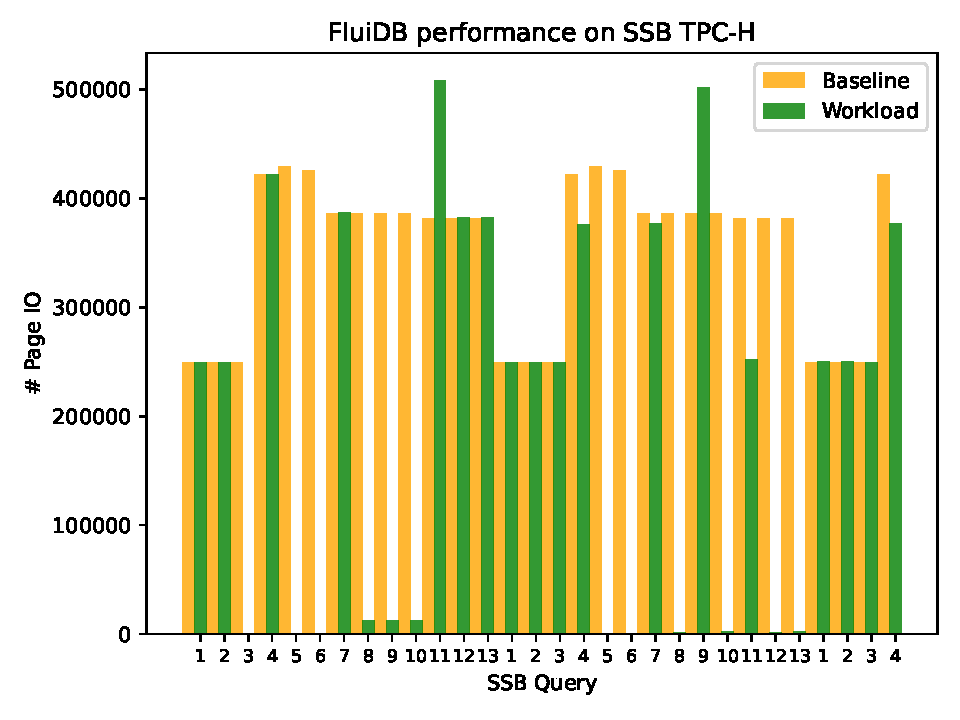
\includegraphics[width=.9\linewidth]{./plans/io_perf_23000.pdf}
  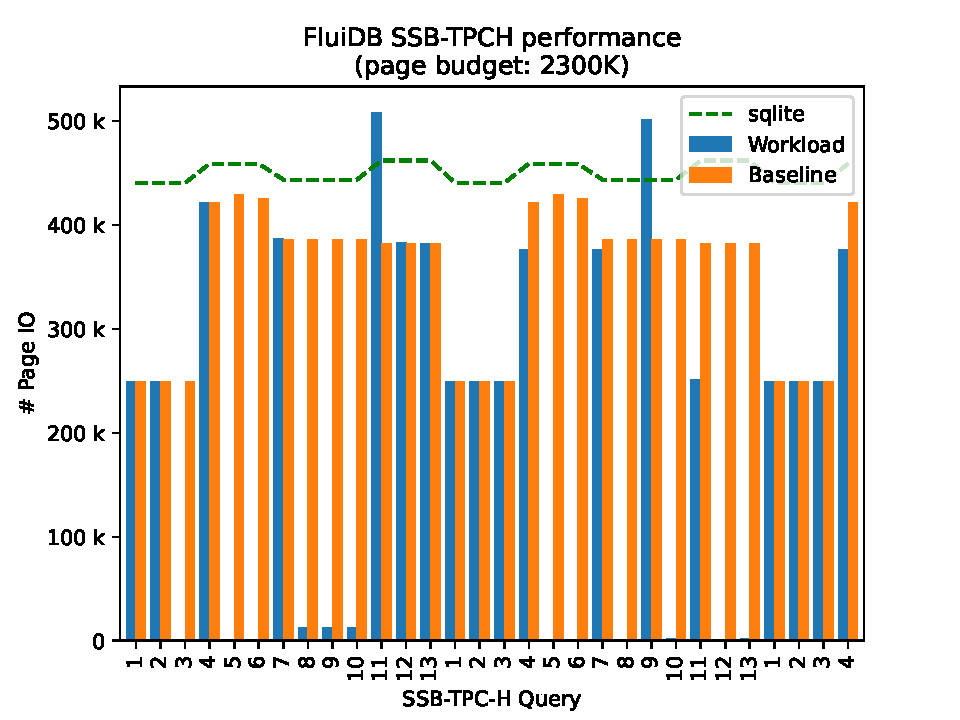
\includegraphics[width=.9\linewidth]{./plans/workload_2300K.pdf}
  \caption{\label{fig:min_budget_plot} \ioperfdescr The budget allowed
    for this is the minimum budget within which FluiDB can run each
    individual query (2300K pages).}
\end{figure}

Figure \ref{fig:min_budget_plot} demonstrates that FluiDB running a
workload versus running each query individually causes speedups even
in constrained budgets. This particular run is run on the minimum
space budget for which the planner is able to create plans for every
individual query. In some cases, however, the garbage collector is
forced to delete tables that need to be recreated later in the
workload causing FluiDB to be sporadically less performant than the
base case.

For a larger budget, the FluiDB is able to store more useful
intermediate results as demonstrated in figure
\ref{fig:large_budget_plot}.

\begin{figure}[H]
  \centering
  % 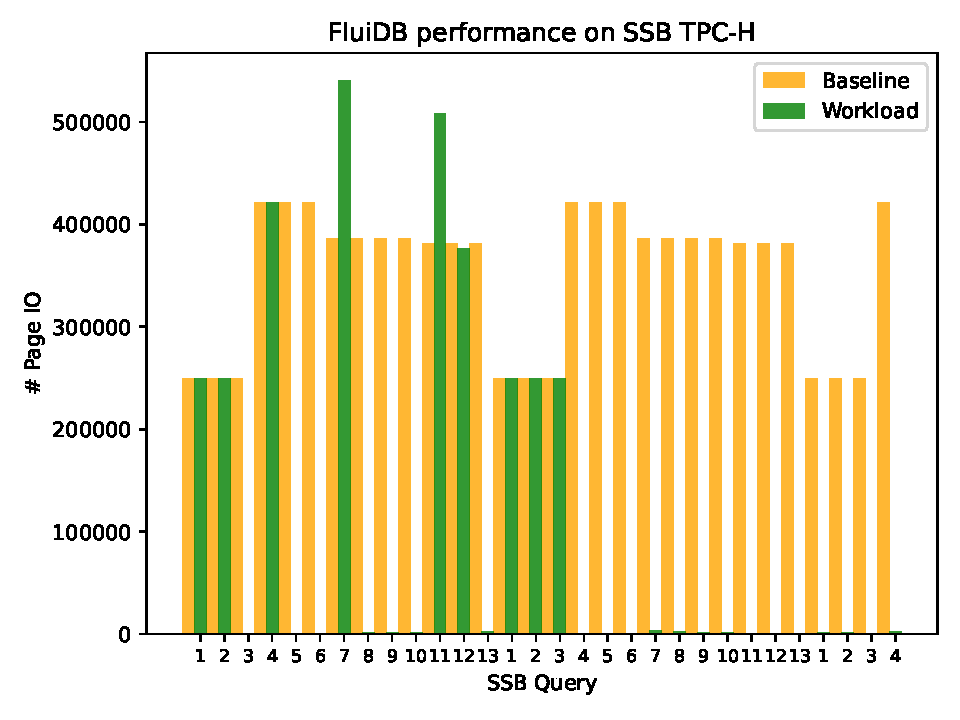
\includegraphics[width=.9\linewidth]{./plans/io_perf_61000.pdf}
  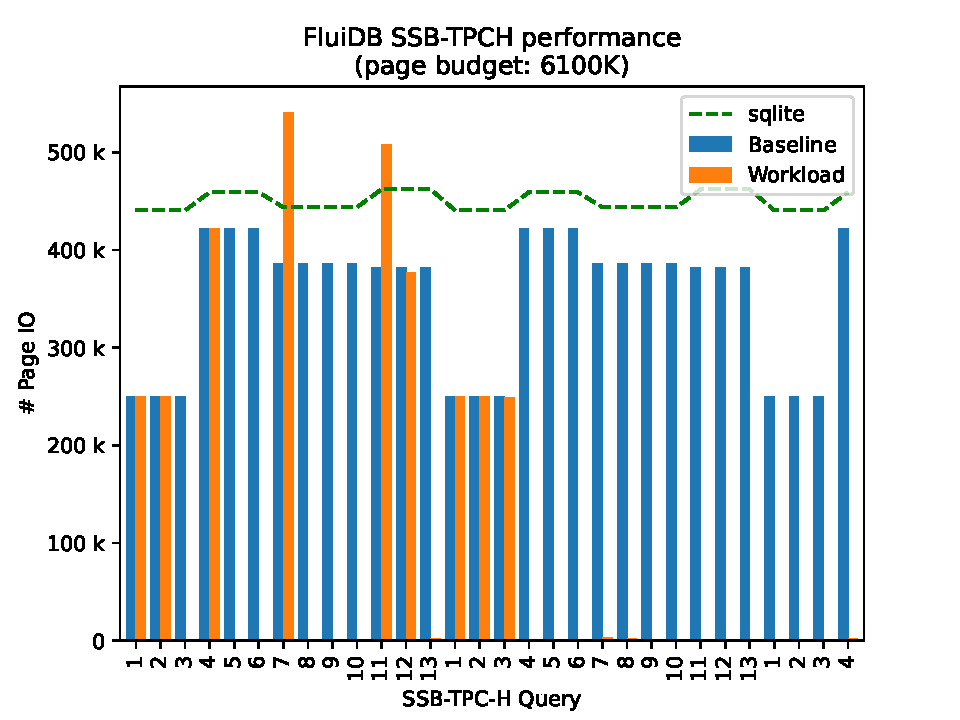
\includegraphics[width=.9\linewidth]{./plans/workload_6100K.pdf}
  \caption{\label{fig:large_budget_plot} \ioperfdescr The budget
    allowed for this is about triple the minimum budget within which
    FluiDB can run each individual query (6100K pages). A badly timed GC
    run causes some individual queries to be slower than their
    counterparts from a workload being run in a tight budget (figure
    \ref{fig:min_budget_plot}).}
\end{figure}

An interesting point here is the plan for evaluating query 7 is more
expensive in the workload run under laxer budgetary constraints. This
may seem strange but it is an example demonstrative of the fundamental
operation of FluiDB. The high level explanation for this is that the
high-budget plan needs to evaluate \(\mathit{lineorder}\) via the
reverse trigger of a join as it was deleted during the evaluation of
query 6. Mysteriously, during the strict-budget planning the
\(\mathit{lineorder}\) relation is readily available during the
planning of query 7! The key lies slightly earlier in the workload
(see listing \ref{fig:reverse_operations_ev}).

FluiDB materializes in query 4 the join

\[
  Q_{36} := \mathit{supplier} \Join_{\mathit{lo\_suppkey} = \mathit{s\_suppkey}} \mathit{lineorder}
\]

and the corresponding antijoins \(Q_{35}\) and \(Q_{37}\), making the
node \(\mathit{lineorder}\) deletable. However, when running the
workload under strict budgetary constraints, it is forced to garbage
collect shortly after materializing said join at a moment while both
\(Q_{36}\) and \(\mathit{lineorder}\) are protected (see section
\ref{sec:gc} on garbage collection). Therefore, FluiDB is forced to
delete both \(Q_{35}\) and \(Q_{37}\), making \(\mathit{lineorder}\)
non-deletable when planning for query 4 finishes.

On the other hand, with laxer budgetary constraints, no garbage
collection is triggered during query 4. The next garbage collection is
triggered during query 6, at a moment when \(\mathit{lineorder}\) is
deletable, unprotected, and a prime candidate for deletion based on
the GC heuristics. Alas, when query 7 requires \(\mathit{lineorder}\)
for its plan, FluiDB needs to reconstruct it in the case of lax
budgetary constraints but not in the case of strict constraints.

This example of FluiDB being forced to locally produce more expensive
plans is an effect of FluiDB being more opportunistic, the lower the
available budget is, and more adventurous when operating with high
budgets. When FluiDB is frugal, it is generally prone to miss
opportunities to share computation between queries. There are times
however that this frugality saves it from bad heuristic-based
decisions that it is allowed to make otherwise.

\begin{code}
\begin{minted}[escapeinside=||,mathescape=true]{trace-lexer.py:TraceLexer -x}
# Query 4
Query |\(s \gamma \pi \sigma (\mathit{supplier} \Join \mathit{lineorder} \Join \mathit{date} \Join \mathit{part})\)| {
  # There is enough space to keep both and the complements
  |\(Q_{36}, Q_{35}, Q_{37}\)| := Materialize[|\(\mathit{supplier} \Join \mathit{lineorder}, \mathit{supplier} \cancel\ltimes \mathit{lineorder}, \mathit{supplier} \cancel\rtimes \mathit{lineorder}\)|]
  |\(Q_{41}, Q_{40}, Q_{42}\)| := Materialize[|\(Q_{36} \Join \mathit{date}, Q_{36} \cancel\ltimes \mathit{date}, Q_{36} \cancel\rtimes \mathit{date}\)|]
  |\(Q_{46}, Q_{45}, Q_{47}\)| := Materialize[|\(Q_{41} \Join \mathit{part}, Q_{41} \cancel\ltimes \mathit{part}, Q_{41} \cancel\rtimes \mathit{part}\)|]
  |\(Q_{50}\)| := Materialize[|\(\sigma Q_{46}\)|]
  |\(Q_{90}\)| := Materialize[|\(\gamma \pi Q_{50}\)|]
  |\(Q_{91}\)| := Materialize[|\(s Q_{90}\)|]
}

# Query 5
Query |\(s \gamma \pi \sigma (\mathit{supplier} \Join \mathit{lineorder} \Join \mathit{date} \Join \mathit{part})\)| {
  |\(Q_{92}\)| := Materialize[|\(\sigma Q_{46}\)|]
  |\(Q_{118}\)| := Materialize[|\(\gamma \pi Q_{92}\)|]
  |\(Q_{119}\)| := Materialize[|\(s Q_{118}\)|]
}

# Query 6
Query |\(s \gamma \pi \sigma (\mathit{supplier} \Join \mathit{lineorder} \Join \mathit{date} \Join \mathit{part}))\)| {
  # FluiDB decides delete lineorder since it has the complements
  GC { Delete[|\(\ldots, \mathit{lineorder}, \ldots \)|] }
  |\(Q_{120}\)| := Materialize[|\(\sigma Q_{46}\)|]
  |\(Q_{146}\)| := Materialize[|\(\gamma \pi Q_{120}\)|]
  |\(Q_{147}\)| := Materialize[|\(s Q_{146}\)|]
}

# Query 7
Query |\(s \gamma \pi \sigma (\mathit{customer} \Join \mathit{date} \Join \mathit{lineorder} \Join \mathit{supplier})\)| {
  # Ooops... this would be avoided if we hadn't deleted lineorder.
  |\(\mathit{lineorder}\)| := Materialize[|\(\bar\pi Q_{36} \cup Q_{37}\)|]
  |\(\mathit{date}\)| := Materialize[|\(\bar\pi Q_{41} \cup Q_{42}\)|]
  GC { Delete[|\( \ldots \)|] }
  |\(Q_{149}, Q_{148}, Q_{150}\)| := Materialize[|\(\mathit{date} \Join \mathit{lineorder}, \mathit{date} \cancel\ltimes \mathit{lineorder}, \mathit{date} \cancel\rtimes \mathit{lineorder}\)|]
  GC { Delete[|\( \ldots \)|] }
  |\(Q_{154}, Q_{153}, Q_{155}\)| := Materialize[|\(\mathit{customer} \Join Q_{149}, \mathit{customer} \cancel\ltimes Q_{149}, \mathit{customer} \cancel\rtimes Q_{149}\)|]
  GC { Delete[|\( \ldots \)|] }
  |\(Q_{165}\)| := Materialize[|\(\sigma Q_{154}\)|]
  |\(Q_{182}, Q_{181}, Q_{183}\)| := Materialize[|\(Q_{165} \Join \mathit{supplier}, Q_{165} \cancel\ltimes \mathit{supplier}, Q_{165} \cancel\rtimes \mathit{supplier}\)|]
  GC { Delete[|\( \ldots \)|] }
  |\(Q_{163}\)| := Materialize[|\(\sigma Q_{182}\)|]
  |\(Q_{203}\)| := Materialize[|\(\gamma \pi Q_{163}\)|]
  |\(Q_{204}\)| := Materialize[|\(s Q_{203}\)|]
}

\end{minted}
  \caption{\label{fig:reverse_operations_ev}Abbreviated version of the
    plans of queries 4 to 7 of SSB TPC-H. This demonstrates how an
    unfortunately timed GC can cause cause FluiDB to make some bad decisions}

\end{code}

FluiDB aspires to deal with the entire workload as if it were planning
a single query. While any decision during the planning of a single
query can be scrapped in the backtracking process, FluiDB is
tragically forced to commit to whatever adventurous or conservative
decisions it makes at the end of every planning iteration, doomed to
pay dearly for every misstep but to reap the rewards of every
insightful choice.

Interestingly, this problem goes away when we run with a budget of
3500k pages (figure \ref{fig:extra_large_budget_plot}) as the GC run
is delayed to a time when other relations are better candidates for
deletion than \(\mathit{lineorder}\). A carefully designed set of
heuristics for the GC should avoid this problem in most cases.

\begin{figure}[p]
  \centering
  % 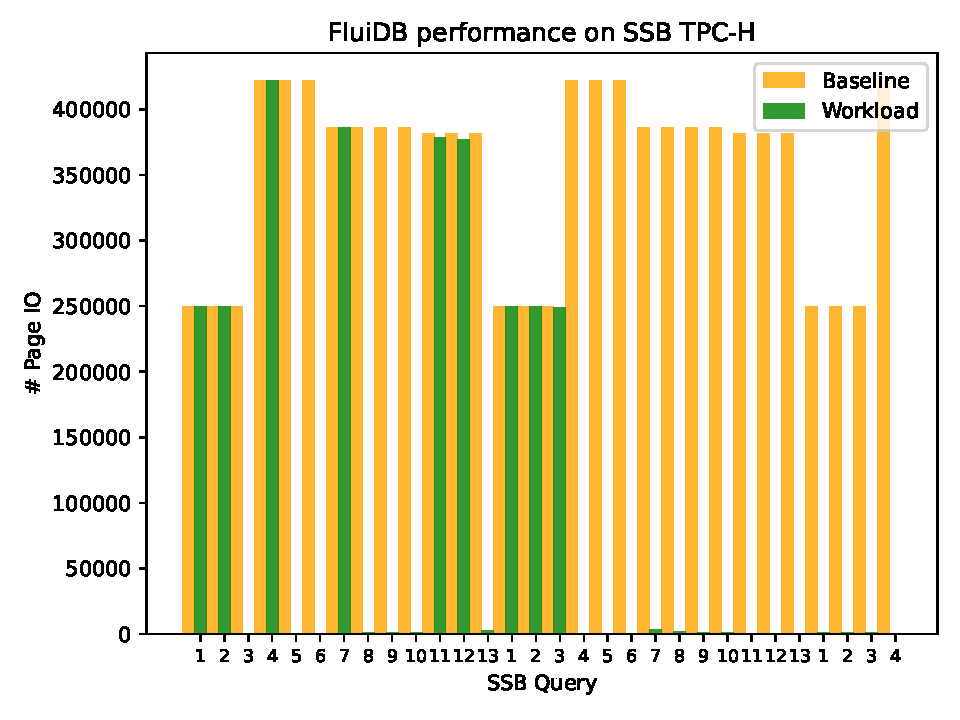
\includegraphics[width=.9\linewidth]{./plans/io_perf_65000.pdf}
  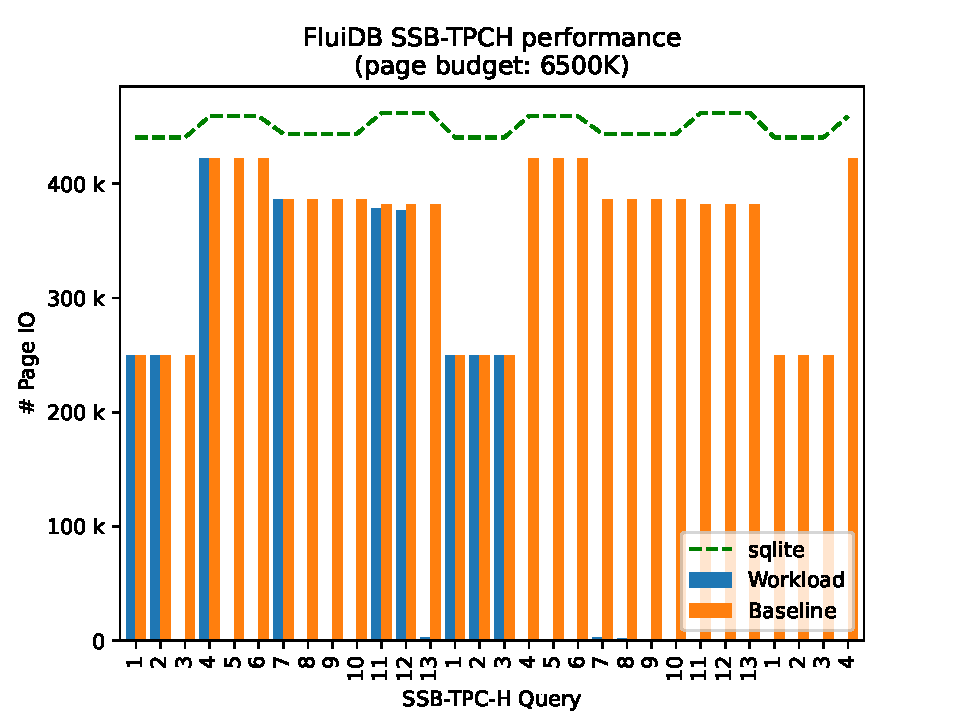
\includegraphics[width=.9\linewidth]{./plans/workload_6500K.pdf}
  \caption{\label{fig:extra_large_budget_plot}
    \ioperfdescr. The budget
    allowed for this is about triple the minimum budget within which
    FluiDB can run each individual query (6500K pages).}
\end{figure}

  It becomes clear from the benchmark results so far that while the GC
  often makes the difference between FluiDB being able to successfully
  run a query and throwing OOM, and while we have put a lot of care in
  tuning it to make good decisions, it can have detrimental effects to
  the performance of the system as a whole. We can't get away from the
  fact that the less the GC is triggered, the less likely it is to
  delete a query useful in the future.

  For that reason, as we discussed in chapter
  \ref{chapter:physical_planning} in detail, FluiDB will only trigger
  the GC when it runs out of memory, and the GC itself goes to great
  lengths to delete as few tables as possible. As demonstrated in
  figure \ref{fig:gc_enemy}, however, the harsh the memory constraints
  will cause the GC not only to run more often it will also be forced
  to evict relations that are likely to be necessary for future
  queries.

  While the GC is a central component of FluiDB, the latter is more than
  a simple cache system as it involves an advanced planner that can
  utilize reversible operations. This means that the search space for
  plans is, in principle, larger than the search space that would be
  available to a recycling RDBMS that does not take advantage of
  reversible operations. As mentioned the performance of FluiDB without
  triggering the GC is demonstrated in figure
  \ref{fig:extra_large_budget_plot}.


  \section{Best/worst case scenarios for FluiDB performance}

  The actual best case scenario for FluiDB is a workload consisting of
  a single query being executed repeatedly. FluiDB will just repeatedly
  return a reference to the table created at the first execution. A
  realistic scenario that is quite good for FluiDB is the presented
  star schema which is the SSB-TPC-H where the number of the possible
  expensive queries (joins) is fairly limited and FluiDB is able to
  eventually figure out which views to materialize and stick with
  them.

  The worst case scenario in the absence of memory constraints is a
  workload that has minimal reuse, the queries that reuse are very far
  apart and therefore no sharing can be exploited. This extreme case
  can be simulated by repeating the schema such that a workload of
  \(N\) queries we would have a repeated \(N\) times TPC-H-SSB schema
  amounting to \(5 \times N\) tables:


  \begin{align*}
    customer_1, date_1 lineorder_1, part_1, supplier_1 \\
    customer_2, date_2 lineorder_2, part_2, supplier_2 \\
    ... \\
    customer_N, date_N lineorder_N, part_N, supplier_N \\
  \end{align*}

  Each query \(Q_i\) will reference tables \(<table>_i\) instead of
  \(<table>\). In terms of the query runtime this is equivalent to
  running each query from scratch each time, i.e. the /"baseline"/ in
  each figure.

  In the presence of constrained memory the more nuanced worst case is
  when the the GC always deletes primary nodes that are needed by the
  next query so each query needs to recreate the primary tables. A
  simple example is:


  \begin{align*}
    Q_1 := lineorder \Join date \Join customer \\
    Q_2 := lineorder \Join part \Join supplier \\
    Q_3 := lineorder \Join date \Join customer \\
    Q_4 := lineorder \Join part \Join supplier \\
    ...
  \end{align*}

  In a memory constrained situation the garbage collector needs to
  delete \(lineorder\) in order to make space for the final join of each
  \(Q_i\), meaning that it needs to recreate \(lineorder\) at each step
  by projecting on \(lineorder \Join part\) for \(Q_{2i + 1}\) and in
  \(lineorder \Join data\) for each \(Q_{2i}\). In slightly more general
  terms this kind of form oscillation that is the worst case workload
  for FluiDB means that every operator in the plan is, not only used
  only once, but needs to be undone. This renders the worst case cost of
  each operator to be its cost + the cost of it's reverse.

  It is hard to compare this case with other databases or even with
  non-GC FluiDB operation because most database systems will fail with
  OOM if their budget can't accommodate all the primary, and every stage
  of intermediate and final relations for the particular workload. While
  this is not a great situation for FluiDB, then, it is in fact much
  better than a failure to resolve the query.

  \begin{figure}[H]
    \centering
    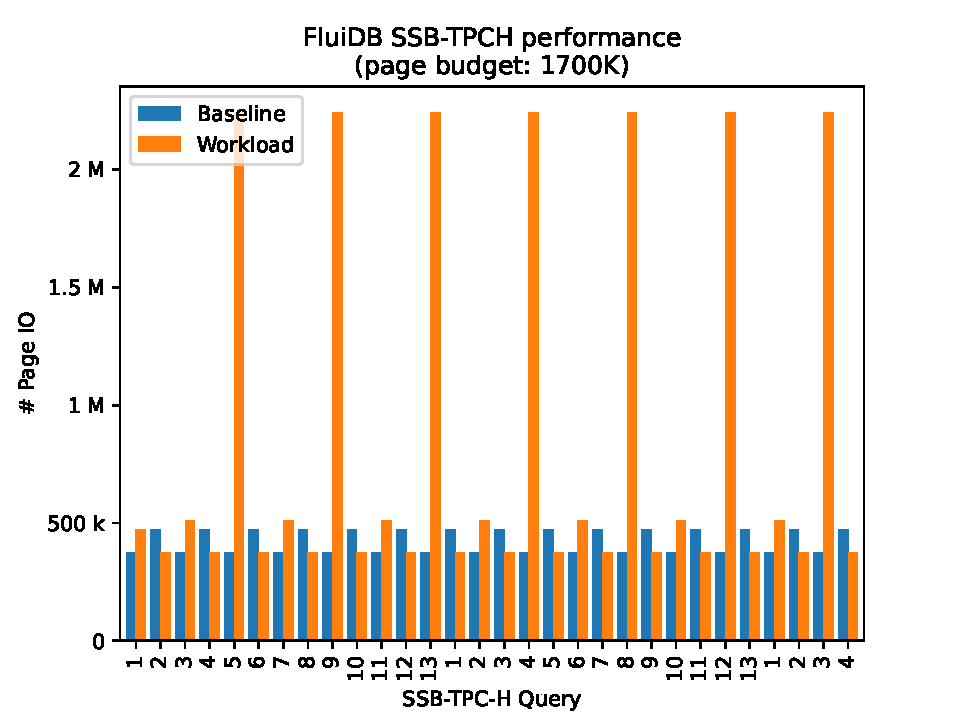
\includegraphics[width=.9\linewidth]{./plans/workload_1700K.pdf}
    \caption{\label{fig:gc_enemy}This plot shows a workload where the GC
      opts to remove primary tables in order to make space for
      intermediate results. The primary tables are then required so they
      need to be reconstructed. The general shape of the queries is
      \(A \Join B_0 \Join C_0\) and \(A \Join B_1 \Join C_1\) and the
      budget is small enough that it can't fit the final result, the
      intermediate result and the primary tables simultaneously. The GC
      is therefore required to delete the primary tables forcing their
      reconstruction the next time it is required.}
  \end{figure}


  The compilation overheads range between a staggering 9 and 11 secs
  per query. While it is not ideal, there are things that can be done
  to mitigate it like prerecompiling the headers (age with the
  \code{-fmodule-header} flag) or changing the granularity of the code
  generation to generate individual operators, which would allow both
  caching of compiled units as well as parallel
  compilation. Optimizing the compilation process itself, however, is
  beyond the scope of this thesis as the overhead is constant (or more
  precisely, a function of the query complexity) and this work focuses
  on optimizing long running queries.

\begin{comment}
  \section{A note on size estimation}
  \label{sec:size_estimation_problems}
  The size of the budget may seem fairly excessive for the size required
  for the primary tables. To understand why that is, we need to look at
  the largest n-nodes in the QDAG:

  \begin{center}
    \begin{tabular}{rl}
      Pages & Expr\\
      \hline
      188000 & \(lineorder\)\\
      547100 & \(customer \Join (date \Join lineorder)\)\\
      376200 & \(\sigma ((customer \Join (date \Join lineorder)) \Join supplier)\)\\
      376200 & \(\sigma ((date \Join lineorder)) \Join supplier)\)\\
      273600 & \(\sigma (customer \Join (date \Join lineorder))\)\\
      188100 & \(\sigma ((\sigma (customer \Join (date \Join lineorder))) \Join supplier)\)\\
    \end{tabular}
  \end{center}

  From looking at those n-nodes it seems that a sufficiently advanced
  garbage collector should be able to support plans that materialize the
  n-nodes in about half the budget as FluiDB should have been able to plan
  the query needing around double the pages required to store the largest equijoin
  which for us is \(customer\) date \(lineorder\).

  The main issue, however, as it is with many query processing systems
  \cite{leisHowGoodAre2015}, is the cardinality estimator which assumes
  that in a natural join there are no foreign key lookup failures, that
  is, that all natural joins are extension joins. Therefore

  \[
    \lvert \sigma _{p(customer)} (customer \Join (date \Join lineorder)) \rvert = \lvert (\sigma _{p(customer)} customer \Join (date \Join lineorder)) \rvert
  \]


  This causes FluiDB to vastly overestimate the size of plans that have
  selections pushed down, making these plans disproportionately
  unappealing.
\end{comment}

\section{Conclusion}

FluiDB is a complex database system built from scratch focused on a
specific idea: making optimal use of the storage budget by fully
adapting the data layout to the workload. While FluiDB is an
experimental system that is probably not stable enough system to be
used in a production setting, it is a complete end-to-end system and
the results presented in this chapter demonstrate that it is based on
ideas worth considering in the design of a commercial database system.
